\documentclass[conference]{IEEEtran}
\usepackage[T1]{fontenc}
\usepackage{amsmath,amssymb,booktabs,graphicx,microtype,url,balance}
\urlstyle{same}
% Shared table typography; no numerical transformations or font scaling.
% Venue classes retain control of captions and manuscript typography.
\usepackage{array,booktabs,tabularx,siunitx}
\sisetup{detect-all,input-ignore={,},group-digits=integer,
  group-separator={,},group-minimum-digits=4}
\newcolumntype{Y}{>{\raggedright\arraybackslash}X}
\newcommand{\pubtable}{\small\centering
  \setlength{\tabcolsep}{4pt}\renewcommand{\arraystretch}{1.16}}
\newcommand{\CI}[2]{\ensuremath{[\num{#1},\,\num{#2}]}}
\newcommand{\estcell}[3]{\shortstack[c]{\num{#1}\\{\footnotesize\CI{#2}{#3}}}}
\newcommand{\thead}[1]{\shortstack[c]{#1}}
\makeatletter
% Expand before alignment starts, so a generated file may begin with a group row.
\newcommand{\tablerows}[1]{\@@input #1 }
\makeatother
\newcommand{\tablenote}[1]{\par\smallskip
  \begin{minipage}{\linewidth}\footnotesize\raggedright #1\end{minipage}}

\newcommand{\dependencyFourChainDelay}{0.583}
\newcommand{\dependencyFourChainInterval}{[0.508, 0.658]}
\newcommand{\dependencyFourChainFee}{8,369.5}
\newcommand{\dependencyFourChainAncestorDelay}{-0.042}
\newcommand{\dependencyFourChainAncestorInterval}{[-0.079, -0.008]}
\newcommand{\dependencyFourChainAncestorFee}{-1,456.775}
\newcommand{\dependencyFaultCount}{8}
\newcommand{\dependencyReplayFixtures}{800}

\newcommand{\dependencyVersionMatchedSets}{751}
\newcommand{\dependencyVersionDifferentSets}{49}
\newcommand{\dependencyVersionFourChainFee}{-1,456.775}
\newcommand{\dependencyVersionFourChainOldGap}{0.646}
\newcommand{\dependencyVersionFourChainNewGap}{1.817}
\newcommand{\dependencyVersionFourStarFee}{-6,139.825}
\newcommand{\dependencyVersionFourStarOldGap}{2.367}
\newcommand{\dependencyVersionFourStarNewGap}{7.208}
\newcommand{\dependencyVersionSixStarFee}{488.4}
\newcommand{\dependencyVersionSixStarOldGap}{0.477}
\newcommand{\dependencyVersionSixStarNewGap}{0.227}

\newcommand{\dependencyExtFourChainRU}{+0.552}
\newcommand{\dependencyExtFourChainRUCI}{[0.508,0.593]}
\newcommand{\dependencyExtFourChainFee}{+8,055}
\newcommand{\dependencyExtFourChainFeeCI}{[5,822,10,431]}
\newcommand{\dependencyExtFourChainGini}{+0.000}
\newcommand{\dependencyExtFourChainGiniCI}{[0.000,0.000]}
\newcommand{\dependencyExtFourChainGap}{-6.9}
\newcommand{\dependencyExtFourChainGapCI}{[-9.0,-5.0]}
\newcommand{\dependencyExtFourStarRU}{+0.560}
\newcommand{\dependencyExtFourStarRUCI}{[0.490,0.630]}
\newcommand{\dependencyExtFourStarFee}{+14,074}
\newcommand{\dependencyExtFourStarFeeCI}{[10,480,17,811]}
\newcommand{\dependencyExtFourStarGini}{+0.010}
\newcommand{\dependencyExtFourStarGiniCI}{[0.003,0.018]}
\newcommand{\dependencyExtFourStarGap}{-11.8}
\newcommand{\dependencyExtFourStarGapCI}{[-15.0,-8.8]}
\newcommand{\dependencyExtSixChainRU}{+0.310}
\newcommand{\dependencyExtSixChainRUCI}{[0.273,0.347]}
\newcommand{\dependencyExtSixChainFee}{+31,009}
\newcommand{\dependencyExtSixChainFeeCI}{[27,286,34,750]}
\newcommand{\dependencyExtSixChainGini}{+0.000}
\newcommand{\dependencyExtSixChainGiniCI}{[0.000,0.000]}
\newcommand{\dependencyExtSixChainGap}{-18.1}
\newcommand{\dependencyExtSixChainGapCI}{[-20.3,-15.8]}
\newcommand{\dependencyDiagEqualSimRU}{+0.550}
\newcommand{\dependencyDiagEqualSimRUCI}{[0.400,0.700]}
\newcommand{\dependencyDiagEqualSimGini}{+0.000}
\newcommand{\dependencyDiagEqualSimGiniCI}{[0.000,0.000]}
\newcommand{\dependencyDiagEqualSimMean}{+0.000}
\newcommand{\dependencyDiagEqualSimMeanCI}{[0.000,0.000]}
\newcommand{\dependencyDiagHeteroSimRU}{-0.150}
\newcommand{\dependencyDiagHeteroSimRUCI}{[-0.300,0.000]}
\newcommand{\dependencyDiagHeteroSimGini}{+0.009}
\newcommand{\dependencyDiagHeteroSimGiniCI}{[0.007,0.011]}
\newcommand{\dependencyDiagHeteroSimMean}{+0.275}
\newcommand{\dependencyDiagHeteroSimMeanCI}{[0.250,0.300]}
\newcommand{\dependencyDiagEqualBatchRU}{+0.317}
\newcommand{\dependencyDiagEqualBatchRUCI}{[0.167,0.450]}
\newcommand{\dependencyDiagEqualBatchGini}{+0.047}
\newcommand{\dependencyDiagEqualBatchGiniCI}{[0.031,0.064]}
\newcommand{\dependencyDiagEqualBatchMean}{+0.025}
\newcommand{\dependencyDiagEqualBatchMeanCI}{[0.000,0.075]}
\newcommand{\dependencyDiagHeteroBatchRU}{-0.683}
\newcommand{\dependencyDiagHeteroBatchRUCI}{[-0.833,-0.533]}
\newcommand{\dependencyDiagHeteroBatchGini}{+0.013}
\newcommand{\dependencyDiagHeteroBatchGiniCI}{[0.006,0.022]}
\newcommand{\dependencyDiagHeteroBatchMean}{+1.075}
\newcommand{\dependencyDiagHeteroBatchMeanCI}{[1.000,1.167]}
\newcommand{\dependencyExtFixtures}{780}
\newcommand{\dependencyExtTrajectories}{2340}
\newcommand{\dependencyExtMILPs}{780}

\newcommand{\ReleaseTimestamp}{2026-11-04 09:24:29 CST (UTC+08:00)}

\title{Who Pays for the Parent?\\Transaction Dependency, Blockspace Allocation, and Confirmation-Delay Redistribution in Bitcoin}
\IEEEoverridecommandlockouts
\author{\IEEEauthorblockN{Anonymous submission\thanks{Code and paper source:\protect\\\protect\url{https://github.com/computational-decision-lab/transaction-dependency-allocation}.\protect\\Full fixtures and data:\protect\\\protect\url{https://huggingface.co/buckets/computational-decision-lab/transaction-dependency-allocation}.}}}
\begin{document}
\maketitle
\pagestyle{plain}
\begin{abstract}
Aggregate delay statistics can conceal a consequential redistribution: CPFP may advance a parent-linked package while postponing unrelated transactions, even when cohort mean delay and Gini do not move. We measure this allocation effect using valid signed transactions in Bitcoin Core v31.0 on Regtest. The original 800 matched fixtures cross twelve equal-weight simultaneous transactions, forty fee assignments, five topologies, and four budgets. In the four-slot chain, Core versus scalar raises unrelated restricted waiting by \dependencyFourChainDelay{} blocks and first-block fees by \dependencyFourChainFee{} sat; against ancestor-package selection, both signs reverse. Mean delay and Gini remain unchanged in these comparisons, as confirmation-count invariance predicts. An actual v30.2 template comparison matches v31.0's initial selected set in 751 of 800 cases. A further 780 fixtures vary size and arrival timing and extend five cells to 100 fee seeds. In the exploratory four-slot chain, heterogeneous sizes reverse the ten-seed unrelated-delay contrast to \dependencyDiagHeteroSimRU{} blocks (95\% interval \dependencyDiagHeteroSimRUCI{}), exposing a boundary of the equal-size finding. Independent reconstruction and official-binary replay check the archived blocks. These controlled results identify a local allocation mechanism; they do not estimate Mainnet delays or user welfare.
\end{abstract}
\begin{IEEEkeywords}
Bitcoin, cluster mempool, CPFP, blockspace allocation, confirmation delay, reproducibility
\end{IEEEkeywords}

\section{Introduction}
Two block builders can report the same aggregate delay while confirming different transactions first. When a transaction spends an unconfirmed parent's output, the parent must precede it in a block. A high-fee child can therefore raise its low-fee parent's effective selection priority and move unrelated transactions to later blocks. If all transactions arrive together and each selector confirms the same number in every block, however, the cohort's mean waiting time and Gini remain identical. Aggregate delay statistics can hide who receives priority.

The economic importance of transaction ordering is established. Fee-market models connect congestion and waiting with user bids and mining incentives~\cite{easley2019,huberman2021}; mechanism-design research studies which payment rules make those incentives compatible~\cite{roughgarden2024,stablefees2023}. Historical Bitcoin evidence also shows that client defaults and major intermediaries shape fee practices~\cite{moser2015}. Kamada and Noda~\cite{kamada2025} jointly model dynamic user bidding and miner operation. Queueing studies derive fee-dependent confirmation times~\cite{kasahara2019,kawase2020}, and a mempool risk-process model links waiting-time distributions to fee choice~\cite{gundlach2024}. These perspectives explain the incentives around blockspace. Reward-instability and mining-gap models allow fees to alter mining behavior~\cite{carlsten2016,tsabary2018}. Our experiment fixes bids and the block schedule to isolate the allocation step: given the same offered fees and transaction weights, which transaction identities obtain scarce space, and what can aggregate delay statistics reveal about that choice?

Child-Pays-For-Parent (CPFP) mechanisms are established practice. Bitcoin Core v31.0 implements cluster mempool: transactions partition into connected components, each linearized into fee-rate chunks that serve as selection units~\cite{bitcoin_core31,core_design31}. Mollakhani, Wuille and Guo study dependency-respecting linearization algorithms and evaluate them on realistic and synthetic mempools~\cite{linearization2026}. We use the pinned v31.0 implementation rather than propose a new algorithm. Our contribution is a controlled downstream allocation benchmark that separates three distinct objects: the priority premium assigned to a selection unit, the displacement of unrelated transactions, and the aggregate confirmation-time distribution.

We construct valid topology interventions by signing new transactions for every graph while matching each label's fee, size, weight, and insertion rank. Three selectors operate on each matched set, and Core generates and validates their blocks. This yields 800 fixtures and 2,400 trajectories, with raw transactions, funding outputs, templates, blocks, and independent reconstruction retained. The resulting benchmark couples an implementation-level comparison with a simple interpretive test: identical per-block confirmation counts must preserve the aggregate burden distribution.

The four-slot chain illustrates why both the benchmark and its comparison rule matter. Relative to scalar selection, Core raises unrelated waiting and first-block fees; relative to ancestor-package selection, both contrasts reverse sign. Aggregate mean waiting and Gini are unchanged in both cases. Priority redistribution therefore has no baseline-free sign, and need not worsen aggregate inequality. Separate replacement trials examine acceptance thresholds as an auxiliary channel distinct from block selection. These findings concern controlled synthetic demand and one node's policy; they do not identify Mainnet miner behavior or user welfare.

\section{Mechanism, estimands and identification}
\subsection{Transactions and feasible allocation}
Let $G=(V,E)$ be the directed acyclic graph of unconfirmed transactions. Transaction $i$ has fee $f_i$, virtual size $v_i$, and weight $w_i$. An edge $(p,c)$ means that $c$ spends an output of $p$. A feasible selected set must contain every unconfirmed ancestor of each selected child and admit a parent-before-child ordering. For transaction-weight budget $W$, feasibility requires
\begin{equation}
 \sum_i w_i x_i\leq W,\qquad x_c\leq x_p\quad\forall(p,c)\in E,
 \qquad x_i\in\{0,1\}.
 \label{eq:feasible}
\end{equation}
Weight and virtual size follow the Segregated Witness definitions~\cite{bip141}. The study's Taproot key-path transactions have no binding sigop adjustment, so raw and policy-adjusted weights coincide. General measurements must distinguish them.

Core partitions a cluster linearization into chunks. A chunk is a selection unit; an entire cluster need not be atomic. At the mempool's initial snapshot, for transaction $i$ in the Core-returned chunk $C_i$, define the dependency premium
\begin{equation}
 DP_i=\frac{4\sum_{j\in C_i} f_j}{\sum_{j\in C_i}w_j}-\frac{f_i}{v_i}.
 \label{eq:dp}
\end{equation}
All experimental weights are divisible by four, so virtual-size rounding differences vanish. The premium is neither a payment to the parent nor a guarantee of next-block inclusion. The allocator recomputes selection after each block; this snapshot measure captures only the initial state.

\subsection{Confirmation and competing outcomes}
For a fixed follow-up horizon $T=8$ scheduled blocks (4,800 seconds) from each transaction's own arrival, let $F_{m,\mathrm{conf}}(t)$ denote confirmation cumulative incidence under selector $m$. Define restricted nonconfirmation time as
\begin{equation}
 R_m(T)=\int_0^T[1-F_{m,\mathrm{conf}}(u)]\,du.
 \label{eq:rnc}
\end{equation}
Here, restricted means truncated at the follow-up horizon. If $a_i$ and $c_i$ are arrival and confirmation times, $B_i=\min(c_i-a_i,T)$; an unconfirmed transaction receives $B_i=T$. The cohort mean equals Eq.~\ref{eq:rnc}. For $n$ transactions and $\bar B>0$, we compute $\mathrm{Gini}=\sum_{i,j}|B_i-B_j|/(2n^2\bar B)$ and report it alongside confirmation incidence. This standard dispersion index~\cite{gastwirth1972} is unchanged by permuting transaction identities. An all-unconfirmed cohort has zero Gini and maximal mean burden, illustrating why inequality alone cannot serve as an efficiency criterion.

The event vocabulary distinguishes confirmation, replacement, expiry, eviction, other removal, unknown removal, and administrative end of observation. Aalen--Johansen estimation retains nonconfirmation removals as competing outcomes~\cite{aalen1978,andersen2012}, rather than treating fee-dependent removals as uninformative censoring. Our selection experiments observe only confirmation and administrative censoring at horizon $T$; separate replacement trials observe replacement and confirmation. We do not claim to have empirically exercised eviction or expiry effects. Replacement concerns the original transaction identifier, not whether a user's payment intent is eventually satisfied by a successor.

Labels 6--11 are disconnected singletons in every matched topology and form the prespecified unrelated cohort $U$. The primary displacement contrast is
\begin{equation}
 DE_U=R_{\mathrm{cluster},U}(T)-R_{\mathrm{scalar},U}(T).
\end{equation}
It can be positive, negative, or zero. A separate topology contrast holds the selector fixed and compares regenerated dependent versus independent graphs. The first changes the selection rule on identical signed transactions; the second changes valid transaction dependencies under matched observable demand. They answer different counterfactual questions.

\subsection{Revenue and utilization}
For each initial mempool, exhaustive enumeration of up to $2^{12}=4096$ subsets yields the exact maximum fee $F^*=\max_{x\text{ satisfying }\eqref{eq:feasible}}\sum_i f_ix_i$. We report selected fees $F_m$, fee capture $F_m/F^*$, its complement $\mathrm{Gap}_m=1-F_m/F^*$, and utilization $\sum_iw_ix_i/W$. With staged arrivals, the optimum uses only transactions already available. This is a first-block revenue benchmark, not a social welfare optimum. Total fees coincide if the entire finite cohort eventually confirms; oversized chunks can prevent that condition under the tested budgets.

\subsection{Why redistribution need not change inequality}
\textbf{Proposition 1 (confirmation-count invariance, standard).} Suppose a fixed cohort arrives simultaneously, block times and the observation horizon are common, and two selectors confirm the same number of transactions in each scheduled block. Then their multisets of restricted burdens are identical, hence their aggregate restricted means and Gini coefficients are equal, even when individual confirmation identities differ.

\emph{Proof.} Each block at time $t_b$ contributes exactly $n_b$ copies of burden $t_b$ to the multiset; transactions not confirmed by $T$ each contribute $T$. The sequence $(n_b,t_b)$ and cohort size fully determine the burden multiset. Both mean and Gini are symmetric functions of that multiset. $\square$

Equal weights and full utilization provide a transparent example. Consider four equal-size transactions with fee rates 2, 100, 40, and 39 sat/vB, where the second spends the first. A two-slot scalar selector initially takes the unrelated transactions at rates 40 and 39; a package selector can take parent plus child at average rate 51. The unrelated transactions each wait one additional block, while the aggregate confirmation-time multiset remains $\{1,1,2,2\}$ blocks. This analytical illustration does not estimate the frequency of such patterns on Bitcoin.

The proposition constrains empirical interpretation. Under simultaneous demand, a change in aggregate delay dispersion requires a change in confirmation counts or competing outcomes, not merely a reordering of identities. Heterogeneous sizes can change those counts. With staggered arrivals, identical calendar-time counts need not preserve the distribution of time since arrival. Our extensions test both boundaries and retain utilization and confirmation incidence alongside Gini.

\section{Executed experimental design}
\subsection{Pinned implementation and local policies}
The reference is Bitcoin Core tag v31.0, commit \texttt{6574cb40869b96b9ffc79c19dc8f4e467d60f321}. We built source with GCC 12.3 and CMake 3.22.1 in Release mode, with wallet enabled and GUI, IPC, and ZMQ disabled. A separately downloaded Linux release binary was checked against its SHA-256 manifest and 13 builder signatures. The archived build manifest records dependency revisions, flags, and binary hashes. This local source build is not claimed to reproduce the Guix release binary byte for byte.

Nodes disable peer networking and bind RPC to loopback. Default cluster limits are retained. Three selectors receive identical signed transactions and transaction-weight budgets:
\begin{enumerate}
\item \emph{Scalar:} Repeatedly select the highest $f_i/v_i$ among transactions whose remaining unconfirmed parents have already been selected; skip transactions that do not fit. Ties use lexicographic transaction identifiers.
\item \emph{Ancestor package:} Recompute each candidate's unselected ancestor package, rank by aggregate fee divided by aggregate virtual size, and select the highest-rate fitting package in topological order. Ties use the candidate identifier. Already-selected ancestors are not counted twice.
\item \emph{Core cluster:} Capture the pinned node's \texttt{getblocktemplate} transaction list. Record \texttt{getmempoolcluster} and \texttt{getmempoolfeeratediagram} outputs but do not substitute a reconstructed cluster order for the actual template.
\end{enumerate}
The first two are declared research policies, not reconstructions of historical miners. An exact rational-rate audit of the original 800 fixtures finds no winning-score tie in 9,600 scalar and 8,770 ancestor-package selection rounds. Transaction-identifier tie breaks therefore do not affect those comparator outcomes; this check does not characterize Core's internal tie handling.

Core's block assembler rejects a chunk if reserved plus transaction weight is \emph{greater than or equal to} its configured maximum. We reserve 2,000 weight units and set the maximum to $2000+W+1$, making the common transaction budget inclusive at $W$. This exact boundary avoids confounding a one-unit implementation detail with topology effects. Sigop limits and minimum relay fees are nonbinding in these fixtures.

\subsection{Valid matched graph construction}
In the original matrix, every transaction uses one input, six Taproot outputs, version two, zero locktime, an explicitly replaceable sequence number, and one fixed-length Schnorr witness. Each is 1,304 weight units and 326 vB. A selected input is funded either by a matured Regtest coinbase UTXO or by a designated parent output. Output values set the exact fee. Every topology is signed anew, decoded, checked with \texttt{testmempoolaccept}, and admitted by Core. Signed bytes are never rewired.

The allocation matrix contains twelve labeled transactions, with labels 0--5 forming the potentially dependent group and 6--11 remaining unrelated. The five graph settings are independent transactions; a two-transaction CPFP pair; a four-transaction chain; a one-parent/five-child star; and a mixed branching component. Forty pseudorandom fee assignments are paired across all graphs and selectors. Label 0 pays 326 sat; label 1 receives the high fee specified by the frozen pseudorandom seed; other labels receive distinct rates drawn from 2--120 sat/vB with small label offsets. The experiment deliberately spans synthetic CPFP incentives and does not fit a Mainnet fee distribution.

For each seed, label-level fees, sizes, weights, and insertion ranks match exactly across graphs. All transactions arrive at a common mock time. Fixed output counts permit legal star and chain variants without changing size. Funding-output values and identifiers change and are retained, but are not modeled utility or user-wealth variables. Every realization passes matching and validity checks before inclusion in the controlled contrast.

Budgets accommodate 2, 4, 6, or 12 transactions per block, yielding 800 graph/seed/budget fixtures and 2,400 selector trajectories. Candidate blocks are generated through Core's \texttt{generateblock}. Raw blocks establish inclusion. Branch invalidation restores the exact signed transaction set between selectors; equal-size distinct coinbase scripts avoid reusing an invalidated block hash. Mock time advances in 600-second steps, so delays are controlled block schedules, not sampled Mainnet block intervals.

The two-slot budget, and some four-slot star cases, are stress conditions: a high-rate chunk may exceed the entire block budget and remain excluded at every subsequent step. Default Mainnet block capacity is much larger than a default cluster size, so this specific permanent-exclusion construction is not presented as a typical Mainnet failure mode. The twelve-slot setting is a no-congestion control. Separate 64- and 65-transaction chains test the cluster-count boundary without entering the twelve-transaction causal matrix.

\subsection{Size, arrival, precision, and version extensions}
An exploratory follow-up adds \dependencyExtFixtures{} fixtures and \dependencyExtTrajectories{} selector trajectories: two size assignments, three arrival schedules, four graphs (independent, CPFP, chain, star), two weight budgets, and ten fee seeds. Heterogeneous sizes are exactly 326, 652, and 1,304 vB, obtained with 6, 13, or 28 Taproot outputs and explicit data padding. Labels have fixed size factors $(1,4,2,1,2,4,1,2,4,1,2,4)$. Fees match by label across topology and size treatments, so changing size also changes fee rates and offered weight. Budgets remain $4\times1304$ or $6\times1304$ WU, not counts of heterogeneous transactions.

All labels arrive at time zero in the simultaneous schedule. In \emph{children-late}, labels 1--5 arrive after the first block; in \emph{two-batch}, labels 3--5 and 9--11 do so. Remaining labels arrive at zero, and no child precedes its parent. Waiting starts at each label's own arrival; a ninth calendar block provides eight-block follow-up for late arrivals. An additional 300 fixtures extend seeds 40--99 for four-unit chain, star, and independent graphs and six-unit chain and independent graphs. Combined with the original forty seeds, these five cells have 100 seed units each. The ten-seed diagnostic reruns are not added as independent precision samples.

We also replay the original 800 signed sets into the official Core v30.2 binary~\cite{bitcoin_core30}, pinned to commit \texttt{4d7d5f6b79d4c11c47e7a828d81296918fd11d4d}. Its checksum and eight builder signatures are verified. Both versions use the same inclusive weight budget; source inspection confirms the same strict capacity boundary. This comparison records actual first-block templates. It does not reconstruct v30 confirmation trajectories or isolate cluster mempool from all other changes between releases.

\subsection{Uncertainty and reproducibility scope}
The repeated unit is the fee-assignment seed. We compute paired differences within each seed and use 10,000 paired bootstrap draws for descriptive 95\% intervals~\cite{efron1979}. Transactions and bootstrap draws do not count as independent replications. Seeds recur across capacities and graphs, so cell estimates are not independent tests. The original surface uses forty seeds, targeted precision cells use 100, and size/arrival diagnostics use ten. Follow-up designs were fixed before their execution but after inspecting the baseline; they are exploratory, without a multiple-testing-adjusted confirmatory or Mainnet sampling claim.

Fresh wallets yield different raw identifiers. Regeneration targets identical label-level fees, sizes, and graphs, with corresponding allocation metrics; captured bytes permit replay of the exact realization. The run retains an initial source snapshot and a recorded orchestration correction that carries mock time across node restarts. Previously completed fixtures were preserved. No treatment configuration was selected or removed in response to an observed outcome.

\section{Results: redistribution and capacity effects}
\subsection{Redistribution without aggregate inequality change}
The independent-transaction controls produce zero differences in measured allocation outcomes across all three selectors at every capacity. In four-slot chain cases, Core minus scalar unrelated-burden contrast is 0.583 blocks (95\% paired-bootstrap interval [0.508, 0.658]), or 350.0 scheduled seconds. First-block fees increase by 8,369.500 sat on average, yet full-cohort mean burden and Gini remain exactly unchanged because each selector still confirms four transactions in each of three blocks. The result is redistribution of which identities wait, as Proposition~1 predicts.

For the child-pays-for-parent pair, the corresponding unrelated contrast is 0.258 blocks [0.208, 0.308]. The mixed graph yields the same aggregate contrasts as the chain for these fee assignments; this does not establish their equivalence under general demand. At six slots, the chain contrast is 0.283 blocks [0.225, 0.342]. Table~\ref{tab:contrasts} and Fig.~\ref{fig:tradeoffs} retain every tested capacity and graph, including null differences. First-block utilization equals one for every policy and cell; capacity stress effects arise in subsequent blocks, not initial weight use.

\subsection{When the capacity constraint changes the distribution}
The four-slot star shows an unrelated contrast of 0.546 blocks ([0.429, 0.667]), a full-cohort mean-burden increase of 0.333 blocks, and a Gini change of +0.0184. Its confirmation-incidence contrast is $-0.0625$. These differences combine identity redistribution with a change in the confirmation-count sequence; some generated star chunks exceed the complete four-slot budget. This is why its aggregate distribution can change while the chain's does not. A high initial dependency premium is insufficient to guarantee inclusion when the selection unit does not fit.

Two-slot cases provide more severe capacity stress. The observed Core minus scalar unrelated means remain nonnegative in these cells, but dependent transactions can also fare worse. In the two-slot star, the parent waits 2.900 more blocks on average under Core despite a positive snapshot dependency premium. A selection unit that cannot fit delivers no priority advantage. This is not evidence that the default Mainnet allocator ordinarily excludes whole clusters indefinitely; the maximum default cluster is far smaller than a default full block.

At twelve slots, all twelve transactions are included in the first block under every selector and graph. Fees and utilization agree, confirmation incidence is one, and restricted-burden Gini is zero. Dependencies can still change the snapshot priority premium but generate no delay contrast when all demand fits. This no-congestion null is part of the result.

\subsection{Topology and algorithm comparisons have different meanings}
The released analysis also holds the Core selector fixed and compares each dependent graph with its newly signed independent-graph counterpart. These paired topology contrasts preserve fees and serialization size but do not hold raw identifiers or UTXO funding values fixed. They are distinct from the Core minus scalar contrasts in the main table. For the four-slot star, the Core topology contrast in unrelated burden is $-0.133$ blocks (interval [-0.263, -0.008]), whereas changing from scalar to Core on the star increases it by 0.546 blocks. The counterfactual therefore changes even the sign of the answer. Against the ancestor comparator on the four-slot chain, the unrelated-burden contrast is $-0.042$ blocks (interval [-0.079, -0.008]), with 1,456.775 fewer first-block satoshis on average. A revenue improvement in one selected block is neither a higher total fee payment by the fixed cohort nor evidence of greater social efficiency.


\subsection{Actual prior-version templates and optimal-fee gaps}
On the original 800 fixtures, v30.2 and v31.0 select identical first-block sets in \dependencyVersionMatchedSets{} cases and different sets in \dependencyVersionDifferentSets{}. In the four-unit chain, the v31.0-minus-v30.2 fee contrast is \dependencyVersionFourChainFee{} sat. Mean optimal-fee gaps are \dependencyVersionFourChainNewGap\% for v31.0 and \dependencyVersionFourChainOldGap\% for v30.2; in the four-unit star they are \dependencyVersionFourStarNewGap\% and \dependencyVersionFourStarOldGap\%. At six units, the star instead favors v31.0 by \dependencyVersionSixStarFee{} sat. These are initial-template results under synthetic budgets, not v30 delay estimates or an isolated causal effect of cluster mempool.

\begin{table*}[t]
\caption{100-seed precision cells: Core cluster minus scalar policy.}
\label{tab:precision_extension}
\pubtable\footnotesize
\begin{tabular*}{\textwidth}{@{\extracolsep{\fill}}r l r c c c c@{}}
\toprule
Budget & Graph & $n$ & {$\Delta R_U$ (blocks)} & {$\Delta F$ (sat)} & {$\Delta G$} & {$\Delta$ gap (pp)}\\\midrule
4 & Chain & 100 & +0.552 [0.508,0.593] & +8,055 [5,822,10,431] & +0.000 & -6.9 \\
4 & Star & 100 & +0.560 [0.490,0.630] & +14,074 [10,480,17,811] & +0.010 & -11.8 \\
6 & Chain & 100 & +0.310 [0.273,0.347] & +31,009 [27,286,34,750] & +0.000 & -18.1 \\
4 & Independent & 100 & +0.000 [0.000,0.000] & +0 [0,0] & +0.000 & +0.0 \\
6 & Independent & 100 & +0.000 [0.000,0.000] & +0 [0,0] & +0.000 & +0.0 \\
\bottomrule

\end{tabular*}
\tablenote{Paired seed-level means and percentile bootstrap intervals; $F$ is first-block fee capture and gap is relative to the exact feasible fee optimum. Five targeted cells combine the original 40 seeds and 60 new seeds. Bootstrap draws are not additional experiments.}
\end{table*}

In the 100-seed four-slot chain, unrelated waiting rises by \dependencyExtFourChainRU{} blocks (95\% interval \dependencyExtFourChainRUCI{}) and first-block fees by \dependencyExtFourChainFee{} sat (\dependencyExtFourChainFeeCI{}), while Gini remains unchanged and the Core-minus-scalar optimal-fee-gap contrast is \dependencyExtFourChainGap{} percentage points. The four-slot star has a Gini increase of \dependencyExtFourStarGini{} and a smaller fee gap; the six-slot chain's unrelated-wait contrast is \dependencyExtSixChainRU{} blocks. Results in Table~\ref{tab:precision_extension} use 100 independent fee seeds per cell.

Ten-seed size/arrival diagnostics show why the original contrast is conditional. In the four-slot chain, Core-minus-scalar unrelated burden changes from \dependencyDiagEqualSimRU{} blocks with equal sizes and simultaneous arrivals to \dependencyDiagHeteroSimRU{} (interval \dependencyDiagHeteroSimRUCI{}) with heterogeneous sizes; the full-cohort Gini contrast becomes \dependencyDiagHeteroSimGini{}. Under two-batch arrivals, the corresponding unrelated contrasts are \dependencyDiagEqualBatchRU{} and \dependencyDiagHeteroBatchRU{} blocks, with Gini contrasts \dependencyDiagEqualBatchGini{} and \dependencyDiagHeteroBatchGini{}. These exploratory cells are small, and their estimates vary jointly with transaction weight, fee rate, and each transaction's age at observation. They delimit the equal-size simultaneous result rather than establish a general effect.

\begin{figure*}[t]
\centering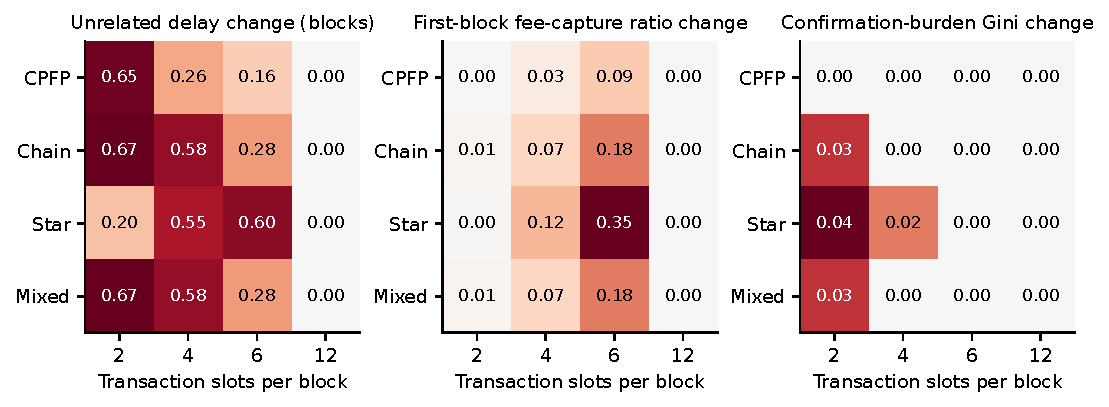
\includegraphics[width=.96\textwidth]{generated/dependency_study/allocation_tradeoffs.pdf}
\caption{Core minus scalar contrasts in the original matrix, averaged over forty paired fee assignments. Time differences are in scheduled blocks. A positive delay contrast means later confirmation for the fixed unrelated cohort. Fee capture is selected fees divided by the exact feasible optimum; it and Gini are dimensionless. First-block utilization is identical in every original cell (Table~\ref{tab:contrasts}). The two-slot column and oversized four-slot star chunks are capacity stress tests; the twelve-slot column is a no-congestion control.}
\label{fig:tradeoffs}
\end{figure*}

\begin{table}[t]
\caption{Core minus scalar: delay and allocation contrasts.}
\label{tab:contrasts}
\pubtable\footnotesize
\setlength{\tabcolsep}{2.5pt}
\begin{tabular*}{\linewidth}{@{\extracolsep{\fill}}r l S[table-format=1.3] c S[table-format=1.3] S[table-format=1.3]@{}}
\toprule
Slots & Graph & {$\Delta R_U$} & 95\% CI & {$\Delta U$} & {$\Delta G$}\\\midrule
\tablerows{generated/dependency_study/contrast_table.tex}
\end{tabular*}
\tablenote{$\Delta R_U$: unrelated restricted delay (blocks); $\Delta U$: first-block utilization; $\Delta G$: full-cohort restricted-burden Gini. Positive differences denote increases under Core. CIs use a paired bootstrap over 40 fee seeds. Two-slot and oversized-chunk four-slot star cases are capacity stress tests.}
\end{table}

\subsection{Replacement acceptance is a separate mechanism}
Block selection is not an RBF rule. Three fixed-shape trials compare Core acceptance with two explicitly defined research replacement policies. Let $D$ be direct conflicts, $R$ conflicts plus their removed descendants, and $A$ retained unconfirmed ancestors. The scalar comparator requires replaceability signaling, no new unconfirmed parents, an eviction cap of 100 transactions, a candidate rate no lower than each direct conflict, and
\begin{equation}
 f_{\mathrm{new}}\geq\sum_{i\in R} f_i+\lceil0.1v_{\mathrm{new}}\rceil.
\end{equation}
The 0.1 sat/vB incremental relay fee is pinned. The ancestor comparator adds
\begin{equation}
 \frac{f_{\mathrm{new}}+\sum_{a\in A}f_a}{v_{\mathrm{new}}+\sum_{a\in A}v_a}
 >\frac{\sum_{i\in R}f_i}{\sum_{i\in R}v_i}.
\end{equation}
BIP125 documents historical opt-in replacement signaling and conditions~\cite{bip125}; neither declared comparator is an exact implementation of that specification or an old Core policy. Core acceptance uses its own fee-rate-diagram rules~\cite{core_replacement31}. Candidate fees are searched at integer-satoshi resolution against a fixed mempool. Adjacent rejection/acceptance checks and a monotonicity grid are archived, followed by actual submission, before/after diagrams, eviction sets, and a mined successor block.

\begin{table}[t]
\caption{Minimum accepted replacement fees (sat).}
\label{tab:rbf}
\pubtable\footnotesize
\begin{tabularx}{\linewidth}{@{}Y *{3}{S[table-format=5.0]}@{}}\toprule
Conflict setting & {Core} & {Scalar} & {Ancestor}\\\midrule
Single 10,000-sat conflict & 10,033 & 10,033 & 10,033\\
\addlinespace[2pt]
Conflict plus 30,000-sat child & 40,033 & 40,033 & 40,033\\
\addlinespace[2pt]
Retained low-fee ancestor & 10,033 & 10,033 & 19,675\\\bottomrule
\end{tabularx}
\tablenote{Each candidate is 326~vB. Core is the pinned implementation; Scalar and Ancestor use the declared research acceptance rules. These three fixtures are deterministic, not population estimates.}
\end{table}
In the third fixture, the 326-sat ancestor also has a 20,000-sat sibling child. The stricter declared ancestor comparator can require a larger fee than Core; the other two cases coincide. Thus the experiment does not support a blanket claim that cluster policy increases replacement costs. For original transaction identifiers that are replaced, confirmation incidence is zero while their restricted burden remains the full follow-up horizon. Treating those removals as uninformative censoring would change the estimand.

\subsection{Policy boundary and independent verification}
The 64-transaction connected fixture is admitted. In the attempted 65-transaction chain, the first 64 transactions are admitted and the last is rejected with \texttt{too-large-cluster}. The rejection is recorded as a policy outcome, not a censored confirmation observation.

The standalone parser imports no Core or generator code. It computes transaction and witness identifiers from raw bytes, derives fees from funding prevouts, calculates weights, extracts graph edges, identifies connected components, aggregates cluster and chunk totals, and verifies fee-rate-diagram concavity. It parses saved blocks, verifies transaction Merkle roots and scheduled timestamps, and reconstructs selected sets and terminal events. A second selector implementation uses fixed-point ancestor closure rather than the generator's recursive package construction. Exhaustive feasible-fee optima are cross-checked with a separate binary mixed-integer linear program solver. Direct event fractions, arithmetic means, and pairwise-distance Gini values cross-check the outcome estimator. Eight deliberate corruptions are rejected: altered fee, truncated transaction, changed signature witness, altered chunk weight, altered delay, duplicate terminal event, early censoring passed to a complete-cohort Gini calculation, and a damaged Merkle root. A closed-form three-outcome example checks competing-risk accounting independently of the selection experiment.

Structural schema checks pass all 800 fixtures. Independent HiGHS binary optimization agrees with exhaustive enumeration on all 800 initial fee optima. A pinned offline container reproduces the reconstructed numerical rows. Wallet-free replay into the separately signed official release binary accepts 9,600 raw transactions and reproduces all 800 initial selected sets with 800 exact order matches. This binary comparison covers the first candidate of every fixture; the standalone parser checks all retained trajectory blocks. Relevant upstream cluster, mempool, miner, RBF, and transaction-graph test suites pass 18 cases and 560,880 assertions; 718 other test cases were skipped. These checks establish captured-input agreement, not a proof of all Core behavior or an independent-laboratory replication.


\section{Related work, interpretation and limits}
The contribution lies between fee-market economics and transaction-graph algorithms. Models of fees and congestion explain the incentives surrounding confirmation~\cite{easley2019,huberman2021,kamada2025}; fee-mechanism design evaluates payment rules and strategic behavior~\cite{roughgarden2024,stablefees2023}. Client-policy evidence shows why concrete implementation choices also matter~\cite{moser2015}. Holding bids and block times fixed lets the present design isolate an allocation mechanism, without inferring equilibrium responses from a change in priority. The comparison with linearization research~\cite{linearization2026} is equally specific: an algorithm's fee-rate ordering does not, by itself, characterize which unrelated transactions wait or whether the cohort's delay dispersion changes. Matched signed graphs, explicit comparators, and confirmation-count invariance make those downstream outcomes separately testable.

Several limits determine the strength of our conclusions. First, twelve-transaction synthetic cohorts, fixed fees, a fixed size assignment, and two staged schedules do not reproduce live traffic or strategic bidding. The size/arrival diagnostics have only ten fee seeds and deliberately stressed weight budgets. Second, candidate templates describe one node's local policy; published mining blocks and network propagation are different observations~\cite{decker2013,gervais2016}, and local policy is distinct from consensus security~\cite{bonneau2015}. Third, oversized chunks can be excluded at the tested budgets; these tail outcomes do not represent typical full blocks. Fourth, transaction Gini is not inequality among identified users, and a replaced identifier is not a user's payment intent. Finally, the eight-block horizon truncates waiting; infinite-horizon outcomes and v30 delay trajectories require additional designs.

Independent replay establishes agreement with the specified binaries on captured inputs and reconstructs the numerical claims. It cannot prove external economic validity, consistent with the distinction between simulation verification and validation~\cite{sargent2013}. Fee capture is not miner profit without accounting for other costs, and waiting time is not a welfare loss without defensible time values and transaction purposes. No Mainnet event history or multi-node observation has been collected for this study. That optional extension has a separate evidence gate and is not silently replaced by Regtest claims.

\balance
\section{Conclusion}
Dependency-aware selection redistributes confirmation priority, but the measured direction depends on the comparator and on size and arrival conditions. In 100-seed equal-size chain cells, unrelated waits rise without a Gini change; small heterogeneous-size diagnostics can reverse that contrast. The evidence remains a single-node, twelve-transaction Regtest benchmark with synthetic fees and constrained budgets. Future work should compare these boundaries with multi-node Mainnet observations and model user bidding before drawing welfare conclusions.

\section*{Reproducibility}
Code, paper source, compact results, signed transaction fixtures, funding blocks, RPC captures, source and binary hashes, configurations, comparators, optimization checks, and reproduction instructions are available through the linked public research repository and data archive. A digest-pinned Python container checks offline numerical reconstruction. This document release was frozen at \ReleaseTimestamp; that timestamp is an artifact identifier, not a Mainnet observation window. Experimental statements are tied to the archived execution and verification artifacts.

\bibliographystyle{IEEEtran}
\bibliography{references}
\end{document}
